\documentclass[11pt]{article}
\usepackage{mathblatt}
% gesetzt von werkzeuge/setzer.py (Sorte selbst) aus dem Lernweg SLM
% und den Bankzeilen; Muster bau/proben/2026-10-09/hypotenuse-muster.
\usepackage{enumitem}
\usepackage{adjustbox,varwidth}
\newgeometry{a4paper,margin=18mm,top=15mm,bottom=20mm,footskip=9mm}
\pagestyle{fancy}\fancyhf{}\renewcommand{\headrulewidth}{0pt}
\fancyfoot[L]{\footnotesize\color{mbgrau}SLM \textperiodcentered{} Wachstum: Faktor und Tabelle}
\fancyfoot[R]{\footnotesize\color{mbgrau}\thepage}
\setlength{\parskip}{3pt}
\renewcommand{\kreuz}[1]{\mbox{$\square$\ #1}\quad}
\newcommand{\kreuzl}[1]{\par\hangindent1.4em\hangafter1\noindent$\square$\ #1}
\newcommand{\aufg}[3]{\par\noindent\makebox[0pt][r]{#3}\begin{minipage}[t]{\linewidth}#1\end{minipage}\par}
\newcommand{\aufgg}[4]{\par\noindent\makebox[0pt][r]{#4}\begin{minipage}[t]{0.6\linewidth}\vspace{0pt}#1\end{minipage}\hfill
  \begin{minipage}[t]{0.37\linewidth}\vspace{0pt}\centering #2\end{minipage}\par}
\newcommand{\nr}[1]{\makebox[7mm][l]{\textbf{#1}}}
\newcommand{\lsg}[3]{\par\noindent\begin{minipage}[t]{9mm}\textbf{#1}\end{minipage}%
  \begin{minipage}[t]{52mm}\raggedright\bfseries\boldmath #2\end{minipage}\hspace{3mm}%
  \begin{minipage}[t]{\dimexpr\linewidth-64mm\relax}\raggedright\small #3\end{minipage}\par\vspace{4pt}}
\newlength{\kr}
\makeatletter
\newcommand{\karomerk}[2]{\protected@write\@auxout{}{\string\karoseite{#1}{#2}{\thepage}}}
\newcommand{\karoseite}[3]{\expandafter\xdef\csname karo@#1@#2\endcsname{#3}}
\newcommand{\karohinweis}[3]{\karomerk{h}{#1}\ifcsname karo@k@#1\endcsname
  \ifnum\csname karo@k@#1\endcsname=0\csname karo@h@#1\endcsname\relax#2\else#3\fi
  \else#3\fi}
\makeatother
\begin{document}

\noindent{\LARGE\bfseries Wachstum: Faktor und Tabelle}\par\smallskip
\noindent{\small\color{mbgrau}Selbstlernheft Klasse 10 \textperiodcentered{} mit Lösungsheft \textperiodcentered{} Kennung SLM}\par\medskip
\noindent\textbf{So nutzt du das Heft:} Lies im Abschnitt das Beispiel. Rechne dann die Aufgaben der Reihe nach und vergleiche jede sofort mit dem Lösungsheft. Kreuze „kann ich“ an, wenn du die letzte Aufgabe (\emph{Ziel}) allein schaffst.\par
\noindent Mehr Aufgaben zu einem Abschnitt: Kennung deinem Nachhilfelehrer schicken (z.\,B. „SLM mehr B“).\par\medskip
{\arrayrulecolor{mbgrau}\renewcommand{\arraystretch}{1.3}
\noindent\begin{tabular}{|>{\bfseries}p{10mm}|p{112mm}|>{\raggedleft\arraybackslash}p{10mm}|>{\centering\arraybackslash}p{14mm}|}\hline
\rowcolor{black!8} & \textbf{Abschnitt} & \textbf{Seite} & \textbf{kann ich}\\\hline
A & Faktor und Prozentsatz & \pageref{s:A} & $\square$\\\hline
B & Faktor aus der Tabelle & \pageref{s:B} & $\square$\\\hline
C & Tabelle fortschreiben & \pageref{s:C} & $\square$\\\hline
D & Zurückrechnen und fehlende Zeit & \pageref{s:D} & $\square$\\\hline
T & Probetest & \pageref{s:T} & $\square$\\\hline
\end{tabular}}\par\bigskip

\begin{tcolorbox}[colback=mbkasten,colframe=mbgrau,boxrule=0.5pt,arc=1mm,left=3mm,right=3mm,top=2mm,bottom=2mm,title={\bfseries Formel auf einen Blick},coltitle=black,colbacktitle=black!10]
\begin{minipage}[t]{0.58\linewidth}\vspace{0pt}
{\Large \large Zunahme um $p\,\%$: \ $q = 1 + \frac{p}{100}$ \par Abnahme um $p\,\%$: \ $q = 1 - \frac{p}{100}$ \par aus der Tabelle: \ $q =$ neuer Wert $:$ alter Wert \par vorwärts: \ Wert $\cdot\, q$, \ $n$ Schritte: Wert $\cdot\, q^n$ \par zurück: \ Wert $:\, q$, \ $n$ Schritte: Wert $:\, q^n$}\par\medskip
In Worten: Der Faktor $q$ sagt, womit du bei jedem Schritt malnimmst. Über $1$ heißt Zunahme, unter $1$ Abnahme.\par\medskip
\textbf{So gehst du vor}\par
\nr{1}Prozentsatz in den Faktor umrechnen oder den Faktor als Quotient aus der Tabelle holen\par
\nr{2}Startwert in den Schritt $0$ schreiben\par
\nr{3}vorwärts mal $q$, über mehrere Schritte mal $q^n$\par
\nr{4}zurück durch $q$\par
\nr{5}fehlende Zeit: mal $q$, bis der Wert passt, Schritte zählen\par
\medskip
{\small Runde erst beim Eintragen: Geld auf Cent, Anzahlen auf ganze Zahlen, sonst auf eine Stelle nach dem Komma. Zwischenwerte nicht runden: Rechne im Taschenrechner mit dem genauen Wert weiter.}
\end{minipage}\hfill
\begin{minipage}[t]{0.38\linewidth}\vspace{2mm}\centering
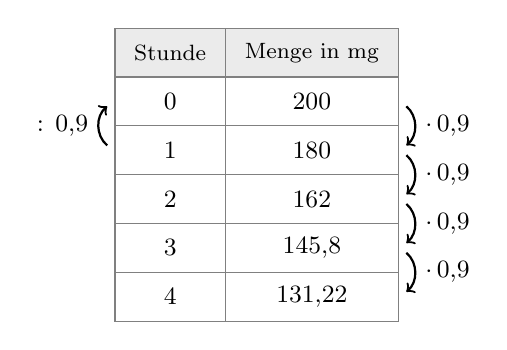
\begin{tikzpicture}[x=1cm,y=-0.62cm,font=\small]\fill[black!8] (0,-1.5) rectangle (3.6,-0.5);\draw[black!50] (0,-1.5) rectangle (1.4,-0.5);\draw[black!50] (1.4,-1.5) rectangle (3.6,-0.5);\node[font=\footnotesize] at (0.7,-1) {Stunde};\node[font=\footnotesize] at (2.5,-1) {Menge in mg};\foreach \zs/\zw [count=\i from 0] in {0/200,1/180,2/162,3/145{,}8,4/131{,}22}{\draw[black!50] (0,\i-0.5) rectangle (1.4,\i+0.5);\draw[black!50] (1.4,\i-0.5) rectangle (3.6,\i+0.5);\node at (0.7,\i) {$\zs$}; \node at (2.5,\i) {$\zw$};}\foreach \i in {0,1,2,3}{\draw[->,thick] (3.7,\i+0.1) to[bend left=50] node[right] {$\cdot\,0{,}9$} (3.7,\i+0.9);}\draw[->,thick] (-0.1,0.9) to[bend left=50] node[left] {$:\,0{,}9$} (-0.1,0.1);\end{tikzpicture}
\end{minipage}
\end{tcolorbox}
\medskip\noindent\textbf{Typische Fehler – so nicht}\par\smallskip
\noindent\nr{$\times$}Den Faktor ohne die Eins gebildet: mal $0{,}05$ statt mal $1{,}05$. Dann schrumpft der Wert, statt zu wachsen.\par
\noindent\nr{$\times$}Differenzen statt Quotienten gebildet, um den Faktor zu finden.\par
\noindent\nr{$\times$}Zurück $4\,\%$ abgezogen: $208 - 4\,\% = 199{,}68$. Richtig: $208 : 1{,}04 = 200$.\par
\noindent\nr{$\times$}$2$ Schritte à $12\,\%$ Abnahme als $24\,\%$ gerechnet. Richtig: $0{,}88 \cdot 0{,}88 = 0{,}7744$, also $22{,}56\,\%$.\par
\clearpage\label{s:A}\noindent\colorbox{black!12}{\makebox[10mm]{\Large\bfseries\strut A}}\hspace{3mm}{\Large\bfseries Faktor und Prozentsatz}\par\smallskip
\noindent Wächst ein Wert um $p\,\%$, rechnest du mal $q = 1 + \frac{p}{100}$; nimmt er um $p\,\%$ ab, mal $q = 1 - \frac{p}{100}$. Den Prozentsatz liest du am Abstand von $q$ zu $1$ ab.\par\medskip
\noindent\textbf{Formel}\par\nopagebreak\noindent\hspace*{4mm}\begin{minipage}{\dimexpr\linewidth-4mm\relax}Zunahme: \ $q = 1 + \frac{p}{100}$ \qquad Abnahme: \ $q = 1 - \frac{p}{100}$ \qquad Prozentsatz: Abstand von $q$ zu $1$\end{minipage}\par\medskip
\noindent\textbf{Beispiel}\quad Gib den Faktor an: a) Eine Miete steigt jedes Jahr um $3\,\%$. b) Ein Akku verliert jeden Monat $4\,\%$ seiner Ladung. Gib den Prozentsatz an: c) Ein Wert wird jedes Jahr mit $0{,}85$ multipliziert. d) Ein Wert wird jedes Jahr mit $1{,}2$ multipliziert.\par\smallskip
\noindent\par\noindent\hangindent6mm\hangafter1\makebox[6mm][l]{\textbf{1}}Zunahme oder Abnahme? „steigt“: Zunahme. „verliert“: Abnahme.\par\smallskip\par\noindent\hangindent6mm\hangafter1\makebox[6mm][l]{\textbf{2}}Zunahme: $q = 1 + \frac{3}{100} = 1{,}03$. Das Komma rückt zwei Stellen nach links: $1{,}9\,\%$ gibt $1 + 0{,}019 = 1{,}019$.\par\smallskip\par\noindent\hangindent6mm\hangafter1\makebox[6mm][l]{\textbf{3}}Abnahme: $q = 1 - \frac{4}{100} = 0{,}96$.\par\smallskip\par\noindent\hangindent6mm\hangafter1\makebox[6mm][l]{\textbf{4}}Vom Faktor zum Prozentsatz: Abstand zu $1$. $0{,}85$ ist kleiner als $1$: $1 - 0{,}85 = 0{,}15$, also $15\,\%$ weniger. $1{,}2$ ist größer als $1$: $1{,}2 - 1 = 0{,}2$, also $20\,\%$ mehr.\par\smallskip\par\medskip
\noindent\textbf{Aufgaben}\hspace{1em}{\small\color{mbgrau}\karohinweis{A}{Rechne unten im Karo.}{Rechne auf einem extra Blatt.} Vergleiche jede Aufgabe gleich mit dem Lösungsheft.}\par\smallskip
\aufg{\hangindent7mm\hangafter1\nr{1.}Gib den Faktor $q$ an. a) Ein Preis steigt um $7\,\%$. b) Ein Bestand sinkt um $7\,\%$. c) Eine Fläche wächst um $40\,\%$. d) Ein Wert nimmt um $2\,\%$ ab.}{}{}
\medskip
\aufg{\hangindent7mm\hangafter1\nr{2.}Gib den Faktor $q$ an. a) Eine Miete steigt um $1{,}9\,\%$. b) Ein Wald verliert $12{,}5\,\%$ seiner Bäume. c) Ein Guthaben wächst um $0{,}5\,\%$. d) Eine Menge halbiert sich.}{}{}
\medskip
\aufg{\hangindent7mm\hangafter1\nr{3.}Ein Wert wird bei jedem Schritt mit dem Faktor multipliziert. Um wie viel Prozent nimmt er zu oder ab? a) $1{,}08$ \ b) $0{,}92$ \ c) $1{,}35$ \ d) $0{,}6$}{}{}
\medskip
\aufg{\hangindent7mm\hangafter1\nr{4.}Vier Banken werben für ein Sparkonto. Kreuze alle Angebote an, bei denen das Guthaben jedes Jahr um $2{,}5\,\%$ wächst.\par\smallskip\leftskip7mm \kreuz{Bank A: $2{,}5\,\%$ Zinsen pro Jahr}\ \kreuz{Bank B: Guthaben jedes Jahr mal $1{,}025$}\par\kreuz{Bank C: Guthaben jedes Jahr mal $1{,}25$}\ \kreuz{Bank D: Guthaben jedes Jahr mal $0{,}975$}}{}{{\scriptsize\color{mbgrau}Ziel\hspace{2mm}}}
\medskip
\par\vspace{3mm}\setlength{\kr}{\dimexpr\pagegoal-\pagetotal-10mm\relax}%
\ifdim\kr>12mm\karomerk{k}{A}\noindent{\scriptsize\color{mbgrau}Platz zum Rechnen}\par\nointerlineskip\vspace{1mm}\noindent
\begin{tikzpicture}\clip (0,0) rectangle ({\linewidth-0.5mm},\kr);\draw[black!16,line width=0.3pt,step=5mm] (0,0) grid (\linewidth,\kr);\end{tikzpicture}\fi\par
\clearpage\label{s:B}\noindent\colorbox{black!12}{\makebox[10mm]{\Large\bfseries\strut B}}\hspace{3mm}{\Large\bfseries Faktor aus der Tabelle}\par\smallskip
\noindent Teile jeden Wert durch den Wert davor. Sind alle Quotienten gleich, ist das der Faktor $q$.\par\medskip
\noindent\textbf{Formel}\par\nopagebreak\noindent\hspace*{4mm}\begin{minipage}{\dimexpr\linewidth-4mm\relax}$q = \text{neuer Wert} : \text{alter Wert}$\end{minipage}\par\medskip
\noindent\textbf{Beispiel}\quad Die Tabelle zeigt die Zahl der Bakterien in einer Probe. Weise nach, dass die Zahl jede Stunde um $30\,\%$ wächst. \newline\adjustbox{max width=\linewidth}{\begin{varwidth}{50cm}\wertetabelle[200,260,338,439{,}4]{\text{Stunde}}{\text{Bakterien in Tausend}}{0,1,2,3}\end{varwidth}}\par\smallskip
\noindent\par\noindent\hangindent6mm\hangafter1\makebox[6mm][l]{\textbf{1}}Quotienten von Wert zu Wert, immer neu $:$ alt: $260 : 200 = 1{,}3$; \ $338 : 260 = 1{,}3$; \ $439{,}4 : 338 = 1{,}3$.\par\smallskip\par\noindent\hangindent6mm\hangafter1\makebox[6mm][l]{\textbf{2}}Alle Quotienten sind gleich, also ist $q = 1{,}3$. Wäre einer anders, wüchse die Zahl nicht jede Stunde um denselben Prozentsatz.\par\smallskip\par\noindent\hangindent6mm\hangafter1\makebox[6mm][l]{\textbf{3}}Prozentsatz: $1{,}3 - 1 = 0{,}3$, also $30\,\%$ mehr.\par\smallskip\par\noindent\hangindent6mm\hangafter1\makebox[6mm][l]{\textbf{4}}Antwort: Jede Stunde wird die Zahl mit $1{,}3$ multipliziert, sie wächst also um $30\,\%$.\par\smallskip\par\medskip
\noindent\textbf{Aufgaben}\hspace{1em}{\small\color{mbgrau}\karohinweis{B}{Rechne unten im Karo.}{Rechne auf einem extra Blatt.} Vergleiche jede Aufgabe gleich mit dem Lösungsheft.}\par\smallskip
\aufg{\hangindent7mm\hangafter1\nr{1.}Die Tabelle zeigt, wie viele Leute ein Video gesehen haben. Bilde die Quotienten. Gib den Faktor und den Prozentsatz an. \newline\adjustbox{max width=\linewidth}{\begin{varwidth}{50cm}\wertetabelle[50,60,72,86{,}4]{\text{Tag}}{\text{Aufrufe in Tausend}}{0,1,2,3}\end{varwidth}}}{}{}
\medskip
\aufg{\hangindent7mm\hangafter1\nr{2.}Die Tabelle zeigt den Wert eines E-Bikes. Bilde die Quotienten. Gib den Faktor und den Prozentsatz an. \newline\adjustbox{max width=\linewidth}{\begin{varwidth}{50cm}\wertetabelle[1\,500,1\,200,960,768]{\text{Jahr}}{\text{Wert in €}}{0,1,2,3}\end{varwidth}}}{}{}
\medskip
\aufg{\hangindent7mm\hangafter1\nr{3.}Die Tabelle zeigt die Zahl der Mitglieder eines Sportvereins. Weise nach, dass die Zahl jedes Jahr um $4\,\%$ gestiegen ist. \newline\adjustbox{max width=\linewidth}{\begin{varwidth}{50cm}\wertetabelle[1\,250,1\,300,1\,352]{\text{Jahr}}{\text{Mitglieder}}{2023,2024,2025}\end{varwidth}}}{}{}
\medskip
\aufg{\hangindent7mm\hangafter1\nr{4.}In der Zeitung steht: „Die Zahl der E-Autos in unserer Stadt wächst jedes Jahr um $25\,\%$.“ Stimmt das für alle Jahre der Tabelle? Begründe. \newline\adjustbox{max width=\linewidth}{\begin{varwidth}{50cm}\wertetabelle[2\,400,3\,000,3\,750,4\,500]{\text{Jahr}}{\text{E-Autos}}{2022,2023,2024,2025}\end{varwidth}}}{}{{\scriptsize\color{mbgrau}Ziel\hspace{2mm}}}
\medskip
\par\vspace{3mm}\setlength{\kr}{\dimexpr\pagegoal-\pagetotal-10mm\relax}%
\ifdim\kr>12mm\karomerk{k}{B}\noindent{\scriptsize\color{mbgrau}Platz zum Rechnen}\par\nointerlineskip\vspace{1mm}\noindent
\begin{tikzpicture}\clip (0,0) rectangle ({\linewidth-0.5mm},\kr);\draw[black!16,line width=0.3pt,step=5mm] (0,0) grid (\linewidth,\kr);\end{tikzpicture}\fi\par
\clearpage\label{s:C}\noindent\colorbox{black!12}{\makebox[10mm]{\Large\bfseries\strut C}}\hspace{3mm}{\Large\bfseries Tabelle fortschreiben}\par\smallskip
\noindent Der Startwert steht im Schritt $0$. Jeder nächste Wert ist der Wert davor mal $q$; über $n$ Schritte rechnest du mal $q^n$.\par\medskip
\noindent\textbf{Formel}\par\nopagebreak\noindent\hspace*{4mm}\begin{minipage}{\dimexpr\linewidth-4mm\relax}nächster Wert $=$ Wert $\cdot\, q$ \qquad nach $n$ Schritten: \ Wert $\cdot\, q^n$\end{minipage}\par\medskip
\noindent\textbf{Beispiel}\quad Auf einem See bedecken Algen zu Beginn $50\,\mathrm{m}^2$. Die Fläche wächst jede Woche um $20\,\%$. Ergänze die Tabelle. \newline\adjustbox{max width=\linewidth}{\begin{varwidth}{50cm}\wertetabelle[,60,,86{,}4,]{\text{Woche}}{\text{Fläche in m²}}{0,1,2,3,6}\end{varwidth}}\par\smallskip
\noindent\par\noindent\hangindent6mm\hangafter1\makebox[6mm][l]{\textbf{1}}Faktor: $20\,\%$ mehr, also $q = 1{,}2$.\par\smallskip\par\noindent\hangindent6mm\hangafter1\makebox[6mm][l]{\textbf{2}}Woche $0$: Der Startwert steht im Text. Trage $50$ ein, ohne zu rechnen.\par\smallskip\par\noindent\hangindent6mm\hangafter1\makebox[6mm][l]{\textbf{3}}Lücke in Woche $2$: $60 \cdot 1{,}2 = 72$. Probe mit dem nächsten Wert: $72 \cdot 1{,}2 = 86{,}4$ \checkmark\par\smallskip\par\noindent\hangindent6mm\hangafter1\makebox[6mm][l]{\textbf{4}}Woche $6$: Schritte zählen, $6 - 3 = 3$. Also $86{,}4 \cdot 1{,}2^3 = 149{,}2992 \approx 149{,}3$. Eintragen: $149{,}3$.\par\smallskip\par\medskip
\noindent\textbf{Aufgaben}\hspace{1em}{\small\color{mbgrau}\karohinweis{C}{Rechne unten im Karo.}{Rechne auf einem extra Blatt.} Vergleiche jede Aufgabe gleich mit dem Lösungsheft.}\par\smallskip
\aufg{\hangindent7mm\hangafter1\nr{1.}Auf einem Sparkonto liegen zu Beginn $2\,000\,€$. Das Guthaben wächst jedes Jahr um $5\,\%$. Ergänze die Tabelle. \newline\adjustbox{max width=\linewidth}{\begin{varwidth}{50cm}\wertetabelle[2\,000,,,]{\text{Jahr}}{\text{Guthaben in €}}{0,1,2,3}\end{varwidth}}}{}{}
\medskip
\aufg{\hangindent7mm\hangafter1\nr{2.}In einem Pool sind zu Beginn $640$ g Chlor. Jeden Tag nimmt die Menge um $25\,\%$ ab. Ergänze die Tabelle. \newline\adjustbox{max width=\linewidth}{\begin{varwidth}{50cm}\wertetabelle[,480,,,]{\text{Tag}}{\text{Chlor in g}}{0,1,2,3,4}\end{varwidth}}}{}{}
\medskip
\aufg{\hangindent7mm\hangafter1\nr{3.}Eine Stadt hat im Jahr $2020$ genau $40\,000$ Einwohner. Die Zahl wächst jedes Jahr um $2\,\%$. Ergänze die Tabelle. \newline\adjustbox{max width=\linewidth}{\begin{varwidth}{50cm}\wertetabelle[40\,000,,,]{\text{Jahr}}{\text{Einwohner}}{2020,2021,2022,2030}\end{varwidth}}}{}{}
\medskip
\aufg{\hangindent7mm\hangafter1\nr{4.}Ein Kalb wiegt bei der Geburt $40$ kg. In den ersten Wochen nimmt es jede Woche um $15\,\%$ zu. Ergänze die Tabelle. Um wie viel kg hat das Kalb in den $8$ Wochen zugenommen? \newline\adjustbox{max width=\linewidth}{\begin{varwidth}{50cm}\wertetabelle[,46,,,]{\text{Woche}}{\text{Masse in kg}}{0,1,2,4,8}\end{varwidth}}}{}{{\scriptsize\color{mbgrau}Ziel\hspace{2mm}}}
\medskip
\par\vspace{3mm}\setlength{\kr}{\dimexpr\pagegoal-\pagetotal-10mm\relax}%
\ifdim\kr>12mm\karomerk{k}{C}\noindent{\scriptsize\color{mbgrau}Platz zum Rechnen}\par\nointerlineskip\vspace{1mm}\noindent
\begin{tikzpicture}\clip (0,0) rectangle ({\linewidth-0.5mm},\kr);\draw[black!16,line width=0.3pt,step=5mm] (0,0) grid (\linewidth,\kr);\end{tikzpicture}\fi\par
\clearpage\label{s:D}\noindent\colorbox{black!12}{\makebox[10mm]{\Large\bfseries\strut D}}\hspace{3mm}{\Large\bfseries Zurückrechnen und fehlende Zeit}\par\smallskip
\noindent Einen Schritt zurück teilst du durch $q$. Fehlt eine Zeit, rechnest du so oft mal $q$, bis der Wert herauskommt, und zählst die Schritte.\par\medskip
\noindent\textbf{Formel}\par\nopagebreak\noindent\hspace*{4mm}\begin{minipage}{\dimexpr\linewidth-4mm\relax}Wert davor $=$ Wert $:\, q$ \qquad $n$ Schritte zurück: \ Wert $:\, q^n$\end{minipage}\par\medskip
\noindent\textbf{Beispiel}\quad Ein Stoff wird abgebaut: Jede Stunde ist $10\,\%$ weniger da. Ergänze die Tabelle. \newline\adjustbox{max width=\linewidth}{\begin{varwidth}{50cm}\wertetabelle[,180,162,131{,}22,]{\text{Stunde}}{\text{Menge in mg}}{0,1,2,?,6}\end{varwidth}}\par\smallskip
\noindent\begin{minipage}[t]{0.6\linewidth}\vspace{0pt}\par\noindent\hangindent6mm\hangafter1\makebox[6mm][l]{\textbf{1}}Faktor: $10\,\%$ weniger, also $q = 0{,}9$. Probe: $162 : 180 = 0{,}9$ \checkmark\par\smallskip\par\noindent\hangindent6mm\hangafter1\makebox[6mm][l]{\textbf{2}}Einen Schritt zurück: durch $q$ teilen. Stunde $0$: $180 : 0{,}9 = 200$. (Zwei Schritte zurück: durch $q^2$, etwa $45 : 1{,}5^2 = 20$. Probe: $20 \cdot 1{,}5^2 = 45$ \checkmark)\par\smallskip\par\noindent\hangindent6mm\hangafter1\makebox[6mm][l]{\textbf{3}}Fehlende Zeit: weiter mal $q$, bis $131{,}22$ herauskommt: $162 \cdot 0{,}9 = 145{,}8$ (Stunde $3$), $145{,}8 \cdot 0{,}9 = 131{,}22$ (Stunde $4$). Es fehlt die $4$.\par\smallskip\par\noindent\hangindent6mm\hangafter1\makebox[6mm][l]{\textbf{4}}Stunde $6$: $200 \cdot 0{,}9^6 = 106{,}288\ldots \approx 106{,}3$.\par\smallskip\end{minipage}\hfill
\begin{minipage}[t]{0.37\linewidth}\vspace{0pt}\centering 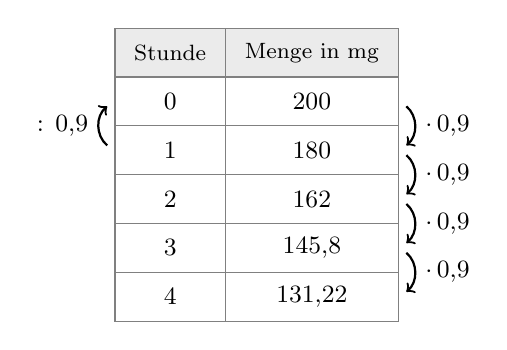
\begin{tikzpicture}[x=1cm,y=-0.62cm,font=\small]\fill[black!8] (0,-1.5) rectangle (3.6,-0.5);\draw[black!50] (0,-1.5) rectangle (1.4,-0.5);\draw[black!50] (1.4,-1.5) rectangle (3.6,-0.5);\node[font=\footnotesize] at (0.7,-1) {Stunde};\node[font=\footnotesize] at (2.5,-1) {Menge in mg};\foreach \zs/\zw [count=\i from 0] in {0/200,1/180,2/162,3/145{,}8,4/131{,}22}{\draw[black!50] (0,\i-0.5) rectangle (1.4,\i+0.5);\draw[black!50] (1.4,\i-0.5) rectangle (3.6,\i+0.5);\node at (0.7,\i) {$\zs$}; \node at (2.5,\i) {$\zw$};}\foreach \i in {0,1,2,3}{\draw[->,thick] (3.7,\i+0.1) to[bend left=50] node[right] {$\cdot\,0{,}9$} (3.7,\i+0.9);}\draw[->,thick] (-0.1,0.9) to[bend left=50] node[left] {$:\,0{,}9$} (-0.1,0.1);\end{tikzpicture}\end{minipage}\par\medskip
\noindent\textbf{Aufgaben}\hspace{1em}{\small\color{mbgrau}\karohinweis{D}{Rechne unten im Karo.}{Rechne auf einem extra Blatt.} Vergleiche jede Aufgabe gleich mit dem Lösungsheft.}\par\smallskip
\aufg{\hangindent7mm\hangafter1\nr{1.}a) Ein Guthaben wächst jedes Jahr um $4\,\%$. Nach einem Jahr sind es $520\,€$. Wie viel war es zu Beginn? b) Ein Auto verliert jedes Jahr $15\,\%$ seines Werts. Nach einem Jahr ist es $17\,000\,€$ wert. Was hat es neu gekostet?}{}{}
\medskip
\aufg{\hangindent7mm\hangafter1\nr{2.}Eine Wasserpflanze bedeckt einen Teich. Ihre Fläche wächst jede Woche um $50\,\%$. In Woche $2$ sind es $45\,\mathrm{m}^2$. Wie groß war die Fläche in Woche $0$?}{}{}
\medskip
\aufg{\hangindent7mm\hangafter1\nr{3.}Die Zahl der Follower eines Kanals wächst jeden Monat um $20\,\%$. In der Tabelle fehlt ein Monat. Welcher Monat gehört dorthin? \newline\adjustbox{max width=\linewidth}{\begin{varwidth}{50cm}\wertetabelle[500,600,1\,036{,}8]{\text{Monat}}{\text{Follower}}{0,1,?}\end{varwidth}}}{}{}
\medskip
\aufg{\hangindent7mm\hangafter1\nr{4.}Ein Patient bekommt ein Schmerzmittel. Jede Stunde baut der Körper $20\,\%$ der Menge ab. a) Wie viel mg hat er zu Beginn bekommen? b) Welche Zeit fehlt in der Tabelle? c) Die Ärztin sagt: „Nach $6$ Stunden ist weniger als ein Viertel der Anfangsmenge übrig.“ Stimmt das? \newline\adjustbox{max width=\linewidth}{\begin{varwidth}{50cm}\wertetabelle[40,32,20{,}48,]{\text{Stunde}}{\text{Menge in mg}}{1,2,?,6}\end{varwidth}}}{}{{\scriptsize\color{mbgrau}Ziel\hspace{2mm}}}
\medskip
\par\vspace{3mm}\setlength{\kr}{\dimexpr\pagegoal-\pagetotal-10mm\relax}%
\ifdim\kr>12mm\karomerk{k}{D}\noindent{\scriptsize\color{mbgrau}Platz zum Rechnen}\par\nointerlineskip\vspace{1mm}\noindent
\begin{tikzpicture}\clip (0,0) rectangle ({\linewidth-0.5mm},\kr);\draw[black!16,line width=0.3pt,step=5mm] (0,0) grid (\linewidth,\kr);\end{tikzpicture}\fi\par
\clearpage\label{s:T}\noindent\colorbox{black!12}{\makebox[10mm]{\Large\bfseries\strut T}}\hspace{3mm}{\Large\bfseries Probetest}\par\smallskip
\noindent Gemischt wie in der Prüfung, ohne Beispiel. Taschenrechner erlaubt. Etwa 20 Minuten.\par\medskip
\noindent\textbf{Aufgaben}\hspace{1em}{\small\color{mbgrau}\karohinweis{T}{Rechne unten im Karo.}{Rechne auf einem extra Blatt.} Vergleiche jede Aufgabe gleich mit dem Lösungsheft.}\par\smallskip
\aufg{\hangindent7mm\hangafter1\nr{1.}Ein Start-up hatte im Jahr $2023$ einen Umsatz von $450\,000\,€$, $2024$ waren es $486\,000\,€$ und $2025$ dann $524\,880\,€$. Weise nach, dass der Umsatz jedes Jahr um $8\,\%$ gestiegen ist.}{}{}
\medskip
\aufg{\hangindent7mm\hangafter1\nr{2.}Eine Miete steigt jedes Jahr um $1{,}8\,\%$. Mit welchem Faktor rechnest du die Miete im nächsten Jahr aus?\par\smallskip\leftskip7mm \kreuz{$1{,}8$}\ \kreuz{$1{,}18$}\par\kreuz{$1{,}018$}\ \kreuz{$0{,}982$}}{}{}
\medskip
\aufg{\hangindent7mm\hangafter1\nr{3.}Die Miete aus Aufgabe $2$ beträgt im Jahr $2026$ genau $700\,€$ im Monat. Ergänze die Tabelle. \newline\adjustbox{max width=\linewidth}{\begin{varwidth}{50cm}\wertetabelle[,,,]{\text{Jahr}}{\text{Miete in €}}{2026,2027,2028,2031}\end{varwidth}}}{}{}
\medskip
\aufg{\hangindent7mm\hangafter1\nr{4.}Der Luftdruck nimmt mit jedem Kilometer Höhe um $12\,\%$ ab. a) Wie groß ist der Luftdruck auf Meereshöhe ($0$ km)? b) Welche Höhe fehlt in der Tabelle? c) Tim sagt: „Von $0$ bis $2$ km sinkt der Luftdruck um $24\,\%$.“ Stimmt das? Begründe. \newline\adjustbox{max width=\linewidth}{\begin{varwidth}{50cm}\wertetabelle[,774{,}4,527{,}7]{\text{Höhe in km}}{\text{Luftdruck in hPa}}{0,2,?}\end{varwidth}}}{}{{\scriptsize\color{mbgrau}Ziel\hspace{2mm}}}
\medskip
\par\vspace{3mm}\setlength{\kr}{\dimexpr\pagegoal-\pagetotal-10mm\relax}%
\ifdim\kr>12mm\karomerk{k}{T}\noindent{\scriptsize\color{mbgrau}Platz zum Rechnen}\par\nointerlineskip\vspace{1mm}\noindent
\begin{tikzpicture}\clip (0,0) rectangle ({\linewidth-0.5mm},\kr);\draw[black!16,line width=0.3pt,step=5mm] (0,0) grid (\linewidth,\kr);\end{tikzpicture}\fi\par
\end{document}
